% !TeX encoding = UTF-8
\documentclass[14pt]{beamer}
\usetheme{metropolis}        
\usepackage{tikz}
\usepackage[utf8]{inputenc}
\usepackage[spanish]{babel}
\usepackage{pgfpages}
%\setbeameroption{show notes}
%\setbeameroption{show notes on second screen=right}

\usepackage{smartdiagram}
\usepackage{qtree}
\usepackage{listings}
\lstset{language=Java,
    basicstyle=\footnotesize\ttfamily,
    keywordstyle=\footnotesize\color{blue}\ttfamily,
}
\usepackage{graphicx}

\definecolor{celeste}{HTML}{5E91AA}
\definecolor{azul}{HTML}{163F54}

\setbeamercolor{head1}{fg=celeste}
\setbeamercolor{title}{fg=celeste}
\setbeamercolor{subtitle}{fg=celeste}
\setbeamercolor{frametitle}{fg=celeste}
\setbeamercolor{structure}{fg=azul}
\setbeamercolor{normal text}{fg=azul}


\title{Programación funcional para la JVM}
\author{Víctor Orozco - @tuxtor}
\institute{Nabenik}
\date{\today}

\begin{document}

\frame{\titlepage}



\begin{frame}{Acerca de}
\begin{figure}
	\centering
	
\includegraphics[width=\linewidth]{Images/fescudos}
\end{figure}

\end{frame}

\begin{frame}{Intro}
    \huge ¿Como me salto la teoria de la computación para programar funcionalmente? - Estudiante 1
\end{frame}

\begin{frame}{Intro}
    \huge ¿Como me salto la teoria de la computación para programar funcionalmente? - Developer 1
\end{frame}

\begin{figure}
    \centering
    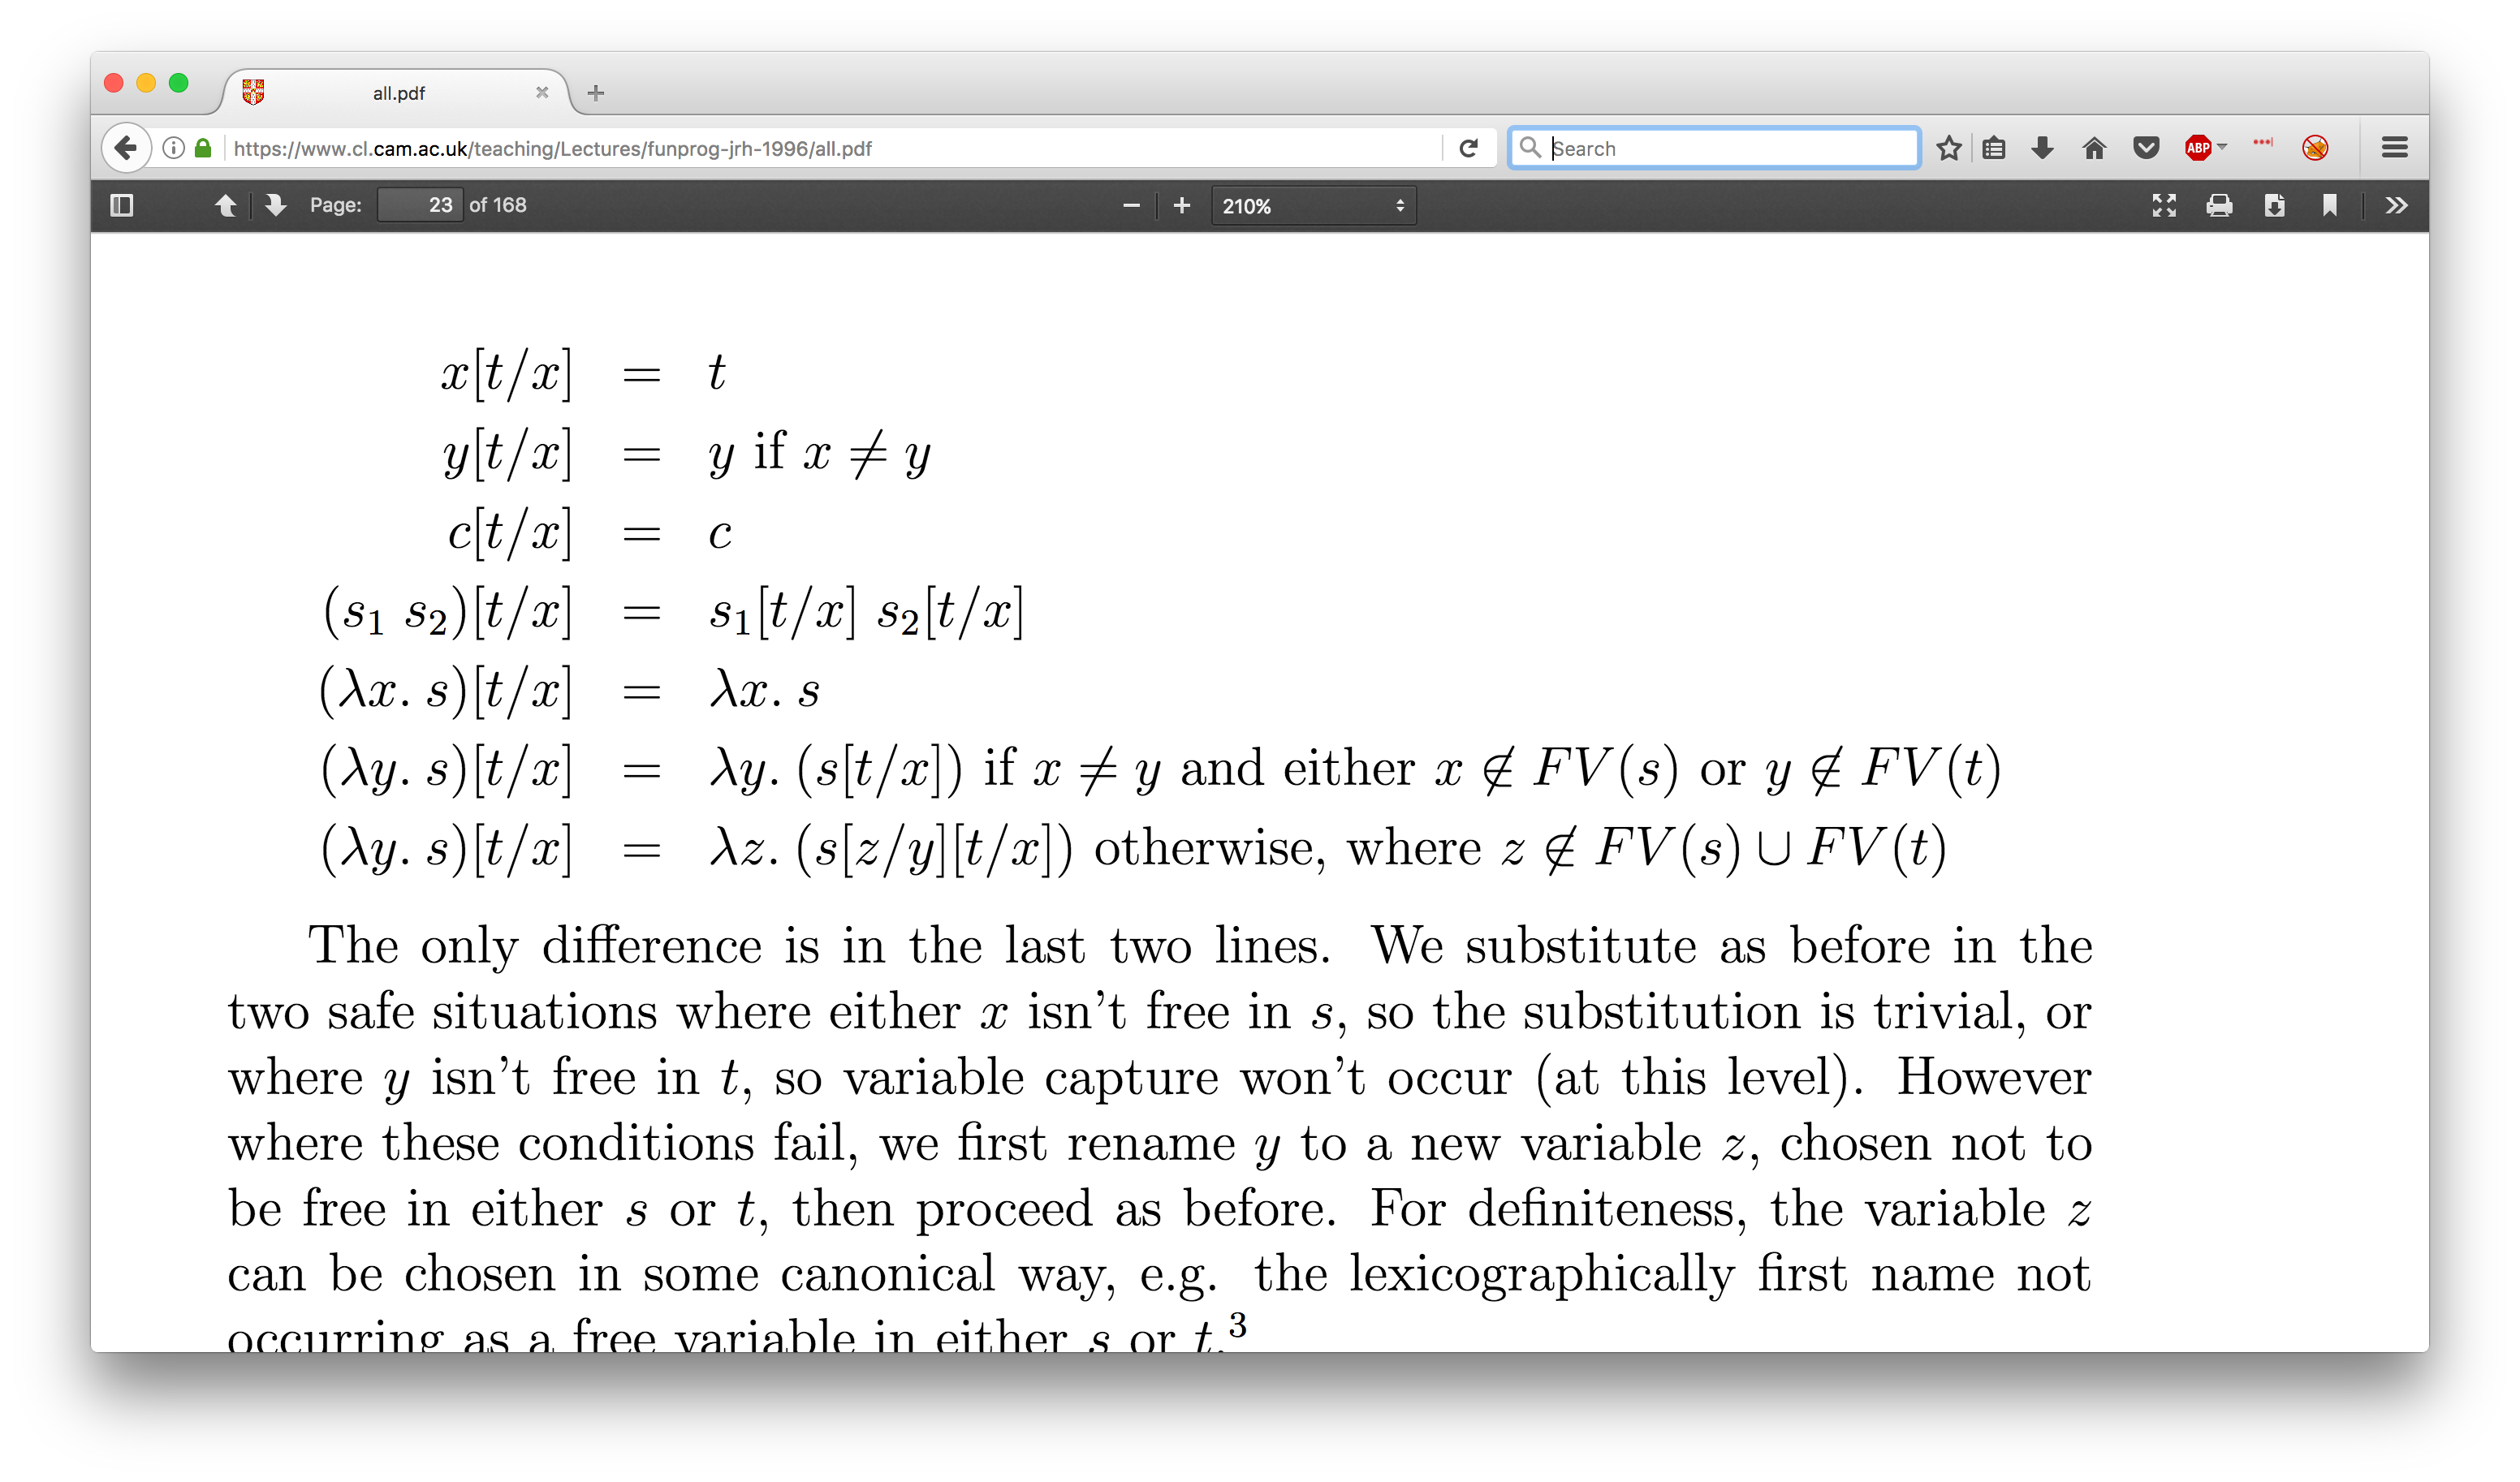
\includegraphics[width=\linewidth]{Images/calculus}
\end{figure}

\begin{frame}{Intro}
    \huge ¿Como aprendo programación funcional?
\end{frame}

\begin{frame}{Intro}
    \huge ¿Que es y como implemento programación funcional?
\end{frame}

 \begin{frame}{Outline}
    \tableofcontents
\end{frame}

\section{Java 8}
\begin{frame}{Java 8}
    2014-03-18 - 3 años!!
    
\href{https://www.oracle.com/java8}{https://www.oracle.com/java8}
\href{https://www.oracle.com/java8launch}{https://www.oracle.com/java8launch}
\end{frame}

\begin{frame}{Java 8}
     \begin{columns}[T] % contents are top vertically aligned
	     \begin{column}[T]{5cm} % each column can also be its own environment
				\begin{itemize}
				\item Nashorn
				\item Date/Time API
				\item Compact Profiles
				\item Type Annotations
				\item \textbf{Default methods}
				\item \textbf{Streams}
				\item \textbf{Lambda Expressions}
				\end{itemize}
	     \end{column}
	     \begin{column}[T]{5cm} % alternative top-align that's better for graphics
			\begin{figure}
			\centering
			
\includegraphics[width=0.7\linewidth]{Images/JavaLam-1}
			\end{figure}

	     \end{column}
     \end{columns}
\end{frame}


\begin{frame}{Paradigmas (Simplificación)}

\Tree[.Paradigmas [.Imperativo [.Estructurado \textit{Pascal} ]
[.OOP  \textit{Java} ]]
[.Declarativo [.Funcional \textit{Clojure} ]
[.Logico \textit{Prolog} ]]]
\end{frame}

\begin{frame}{Programación funcional}
\begin{itemize}
\item Computación = Evaluación de funciones matemáticas (calculo de lambdas)
\item NO cambios en estado
\item NO mutar datos
\item Declarativo $\to$ Expresiones 
\end{itemize}
\end{frame}

\begin{frame}{POO vs. Funcional (organización)}
\smartdiagram[descriptive diagram]{
{POO,{Clases}},
{FP, {Funciones}}}
\end{frame}

\begin{frame}{POO vs. Functional (organization - think about)}
	\smartdiagram[descriptive diagram]{
	  {POO,{Classes}},
	  {FP, {Functions}}}
\end{frame}

\begin{frame}{POO vs. Funcional (algoritmos)}
\smartdiagram[descriptive diagram]{
	{POO,{Imperativo, comportamiento como una serie de pasos}},
	{FP, {Declarativo, interacción de funciones sin especificar su contenido}}}
\end{frame}

\begin{frame}{POO vs. Funcional (Mutabilidad y estado)}
\smartdiagram[descriptive diagram]{
{POO,{Estado y comportamiento juntos, promueve mutabilidad}},
{FP, {Evita estado, promueve inmutabilidad}}}
\end{frame}

\begin{frame}{POO vs. Funcional (Estilo)}
\smartdiagram[descriptive diagram]{
{POO,{OOP + Patrones para abstracciones de alto nivel}},
{FP, {Es una abstracción en alto nivel por si mismo}}}
\end{frame}

\begin{frame}{POO vs. Funcional (Concurrencia)}
\smartdiagram[descriptive diagram]{
{POO,{Concurrencia basica con locks y recursos compartidos}},
{FP, {Workflows paralelos sin estado compartido (no locks!)}}}
\end{frame}

\begin{frame}{POO vs. Funcional (Código)}
\smartdiagram[descriptive diagram]{
{POO,{Descriptivo (demasiado)}},
{FP, {Conciso y denso}}}
\end{frame}

\section{FP}

\begin{frame}{¿Porque programación funcional?}
\begin{itemize}
	\item Paralelismo
	\item Multicore, multicpu
	\item Elegancia
\end{itemize}
\end{frame}

\begin{frame}{Programación funcional en la JVM}
\begin{itemize}
\item Java no es un lenguaje funcional puro (Clojure)
\item Otras opciones JVM (Scala, Kotlin, Ceylon)
\item Java soporta programación funcional a través de bibliotecas
\end{itemize}
\end{frame}


\begin{frame}{Java 8}
Un lenguaje de programación multiparadigma con presencia fuerte de POO con complementos funcionales y orientados a aspectos
\begin{figure}
	\centering
	
\includegraphics[width=0.5\linewidth]{Images/JavaLam-1}
\end{figure}
\end{frame}

\begin{frame}{Kotlin}
Un lenguaje de programación multiparadigma con presencia fuerte de programación funcional con complementos POO
\begin{figure}
	\centering
	
\includegraphics[width=0.5\linewidth]{Images/kotlin}
\end{figure}
\end{frame}

\section{Bloques}

\begin{frame}{Bloques funcionales en Java 8}
\begin{itemize}
\item Interfaces funcionales
\item Referencia a funciones
\item Lambdas
\item Funciones predefinidas en Java 8 (java.util.function)
\item Streams API
\end{itemize}
\end{frame}


\begin{frame}{Bloques funcionales en Kotlin}
\begin{itemize}
	\item Funciones y referencia a funciones
	\item Sintaxis Kotlin
	\item Lambdas
	\item Funciones predefinidas en Kotlin
	\item Streams API
\end{itemize}
\end{frame}


\begin{frame}[fragile]{Streams API}
\begin{itemize}
	\item Map-Reduce
	\item Monads = Serie de pasos / funciones anidadas
\end{itemize}

\smartdiagram[sequence diagram]{Stream,Ops. intermedias,Operación terminal}
\end{frame}

\section{Demo Java y Kotlin}

\section{Fin}
\begin{frame}{Gracias}
\begin{itemize}
	\item me@vorozco.com
	\item http://vorozco.com
	\item http://github.com/tuxtor/slides
\end{itemize}
\begin{center}
	
\includegraphics[width=0.1\linewidth]{Images/cclogo}
	\\
	This work is licensed under a Creative Commons Attribution-ShareAlike 3.0 Guatemala License.
\end{center}
\end{frame}
\end{document}

